\documentclass[tikz, border=10pt]{standalone}
\usepackage{tikz}
\usepackage{amsmath}
\usetikzlibrary{shapes, calc, backgrounds, arrows.meta}

\begin{document}
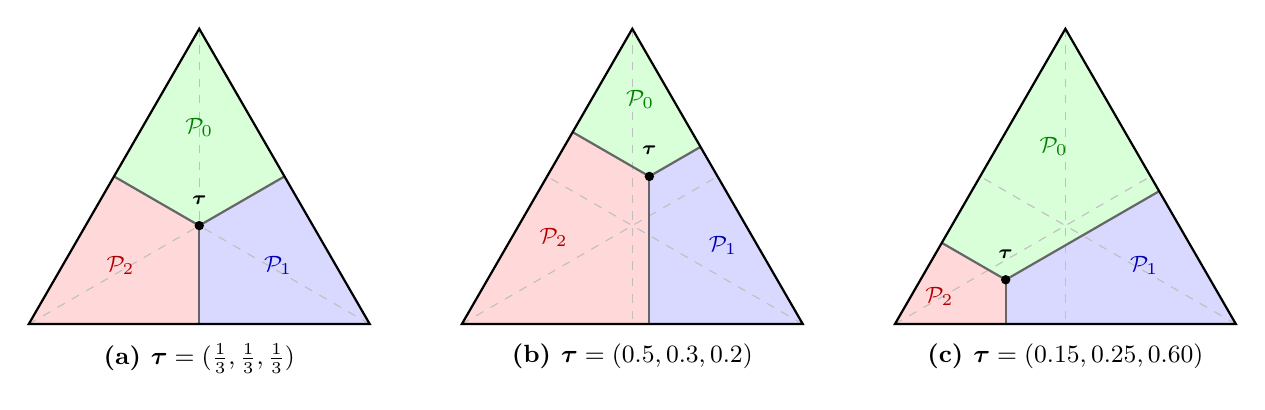
\begin{tikzpicture}[font=\sffamily]

    \begin{scope}[xshift=0.0cm, scale=0.5]
    \coordinate (Top) at (0.000, 5.000);
    \coordinate (Right) at (4.330, -2.500);
    \coordinate (Left) at (-4.330, -2.500);

    \coordinate (Int) at (0.000, 0.000);

    \fill[green!15] (0.000, 5.000) -- (2.165, 1.250) -- (0.000, 0.000) -- (-2.165, 1.250) -- cycle;
    \fill[blue!15] (4.330, -2.500) -- (0.000, -2.500) -- (0.000, 0.000) -- (2.165, 1.250) -- cycle;
    \fill[red!15] (-4.330, -2.500) -- (-2.165, 1.250) -- (0.000, 0.000) -- (0.000, -2.500) -- cycle;

    \draw[dashed, gray!50, thin] (Left) -- (2.165, 1.250);
    \draw[dashed, gray!50, thin] (Right) -- (-2.165, 1.250);
    \draw[dashed, gray!50, thin] (Top) -- (0.000, -2.500);

    \draw[thick, black!60] (Int) -- (2.165, 1.250);
    \draw[thick, black!60] (Int) -- (-2.165, 1.250);
    \draw[thick, black!60] (Int) -- (0.000, -2.500);

    \node[circle, fill=black, inner sep=1.2pt] at (Int) {};
    \node[font=\scriptsize, anchor=south] at (0.000, 0.300) {$\boldsymbol{\tau}$};

    \draw[thick] (Top) -- (Right) -- (Left) -- cycle;

    \node[green!50!black, font=\footnotesize\bfseries] at (0.000, 2.500) {$\mathcal{P}_0$};
    \node[blue!70!black, font=\footnotesize\bfseries] at (2.000, -1.000) {$\mathcal{P}_1$};
    \node[red!70!black, font=\footnotesize\bfseries] at (-2.000, -1.000) {$\mathcal{P}_2$};

    \node[font=\small\bfseries, anchor=north, align=center] at (0, -2.750) {(a) $\boldsymbol{\tau} = (\tfrac{1}{3},\tfrac{1}{3},\tfrac{1}{3})$};
    \end{scope}

    \begin{scope}[xshift=5.5cm, scale=0.5]
    \coordinate (Top) at (0.000, 5.000);
    \coordinate (Right) at (4.330, -2.500);
    \coordinate (Left) at (-4.330, -2.500);

    \coordinate (Int) at (0.433, 1.250);

    \fill[green!15] (0.000, 5.000) -- (1.732, 2.000) -- (0.433, 1.250) -- (-1.516, 2.375) -- cycle;
    \fill[blue!15] (4.330, -2.500) -- (0.433, -2.500) -- (0.433, 1.250) -- (1.732, 2.000) -- cycle;
    \fill[red!15] (-4.330, -2.500) -- (-1.516, 2.375) -- (0.433, 1.250) -- (0.433, -2.500) -- cycle;

    \draw[dashed, gray!50, thin] (Left) -- (2.165, 1.250);
    \draw[dashed, gray!50, thin] (Right) -- (-2.165, 1.250);
    \draw[dashed, gray!50, thin] (Top) -- (0.000, -2.500);

    \draw[thick, black!60] (Int) -- (1.732, 2.000);
    \draw[thick, black!60] (Int) -- (-1.516, 2.375);
    \draw[thick, black!60] (Int) -- (0.433, -2.500);

    \node[circle, fill=black, inner sep=1.2pt] at (Int) {};
    \node[font=\scriptsize, anchor=south] at (0.433, 1.550) {$\boldsymbol{\tau}$};

    \draw[thick] (Top) -- (Right) -- (Left) -- cycle;

    \node[green!50!black, font=\footnotesize\bfseries] at (0.200, 3.200) {$\mathcal{P}_0$};
    \node[blue!70!black, font=\footnotesize\bfseries] at (2.300, -0.500) {$\mathcal{P}_1$};
    \node[red!70!black, font=\footnotesize\bfseries] at (-2.000, -0.300) {$\mathcal{P}_2$};

    \node[font=\small\bfseries, anchor=north, align=center] at (0, -2.750) {(b) $\boldsymbol{\tau} = (0.5, 0.3, 0.2)$};
    \end{scope}

    \begin{scope}[xshift=11.0cm, scale=0.5]
    \coordinate (Top) at (0.000, 5.000);
    \coordinate (Right) at (4.330, -2.500);
    \coordinate (Left) at (-4.330, -2.500);

    \coordinate (Int) at (-1.516, -1.375);

    \fill[green!15] (0.000, 5.000) -- (2.382, 0.875) -- (-1.516, -1.375) -- (-3.139, -0.438) -- cycle;
    \fill[blue!15] (4.330, -2.500) -- (-1.516, -2.500) -- (-1.516, -1.375) -- (2.382, 0.875) -- cycle;
    \fill[red!15] (-4.330, -2.500) -- (-3.139, -0.438) -- (-1.516, -1.375) -- (-1.516, -2.500) -- cycle;

    \draw[dashed, gray!50, thin] (Left) -- (2.165, 1.250);
    \draw[dashed, gray!50, thin] (Right) -- (-2.165, 1.250);
    \draw[dashed, gray!50, thin] (Top) -- (0.000, -2.500);

    \draw[thick, black!60] (Int) -- (2.382, 0.875);
    \draw[thick, black!60] (Int) -- (-3.139, -0.438);
    \draw[thick, black!60] (Int) -- (-1.516, -2.500);

    \node[circle, fill=black, inner sep=1.2pt] at (Int) {};
    \node[font=\scriptsize, anchor=south] at (-1.516, -1.075) {$\boldsymbol{\tau}$};

    \draw[thick] (Top) -- (Right) -- (Left) -- cycle;

    \node[green!50!black, font=\footnotesize\bfseries] at (-0.300, 2.000) {$\mathcal{P}_0$};
    \node[blue!70!black, font=\footnotesize\bfseries] at (2.000, -1.000) {$\mathcal{P}_1$};
    \node[red!70!black, font=\footnotesize\bfseries] at (-3.200, -1.800) {$\mathcal{P}_2$};

    \node[font=\small\bfseries, anchor=north, align=center] at (0, -2.750) {(c) $\boldsymbol{\tau} = (0.15, 0.25, 0.60)$};
    \end{scope}

\end{tikzpicture}
\end{document}
